%!Tex Root = ../Tutorat4.tex
% ./Packete.tex
% ./Design.tex
% ./Deklarationen.tex
% ./Aufgabe2.tex
% ./Aufgabe3.tex
% ./Bonus.tex

\section{Task 1}

\setcounter{task}{1}

\begin{frame}[allowframebreaks]{Task 1}{Earliest Deadline First (EDF) and Total Bandwidth Server (TBS)}
  \begin{tasknoinc}
    \centering
    % 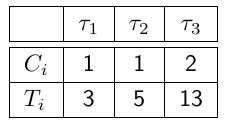
\includegraphics[width=0.25\textwidth]{./figures/1_tasks.png}
      \begin{NiceTabular}{X[1,c]X[2,c]X[2,c]X[2,c]}[rules/color=SecondaryColor] % {\linewidth}{|C|C|L|L|}
        \CodeBefore
        \chessboardcolors{white}{BoxColor}
        \rowcolor{SecondaryColor}{1}
        \columncolor{SecondaryColor}{1}
        \Body
        & \textcolor{white}{$\tau_1$} & \textcolor{white}{$\tau_2$} & \textcolor{white}{$\tau_3$} \\
        \textcolor{white}{$C_i$} & 1 & 1 & 2 \\
        \textcolor{white}{$T_i$} & 3 & 5 & 13 \\
        \bottomrule
      \end{NiceTabular}
    \begin{itemize}
      \item \alert{TBS} executes along with the \alert{periodic tasks} above
      \item what can be the maximum value of $U_s$ such that the whole set (i.e. periodic tasks and the \alert{TBS}) is schedulable with \alert{EDF}?
    \end{itemize}
  \end{tasknoinc}
  \begin{requirementsnoinc}
    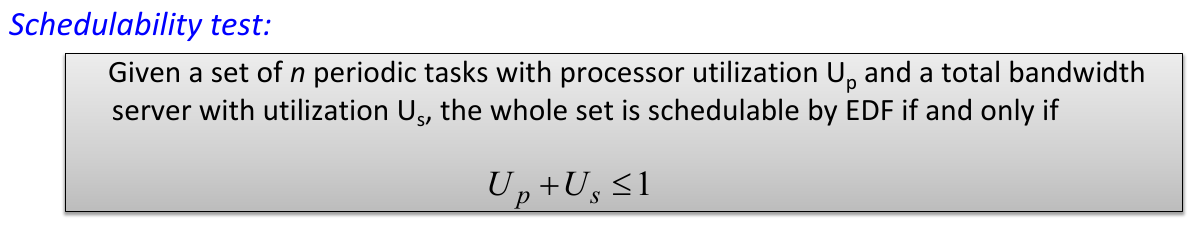
\includegraphics[width=\textwidth]{./figures/schedulability_test.png}
    \begin{itemize}
      \item \alert{processor utilization factor:} $\displaystyle U=\sum_{i=1}^n \frac{C_i}{T_i}$
    \end{itemize}
  \end{requirementsnoinc}
  \begin{solution}
    \begin{itemize}
      \item \alert{Maximum utilization of the Total Bandwidth Server:} $U_{s, \max }=1-U_p=1-(\frac{1}{3}+\frac{1}{5}+\frac{2}{13})=\frac{61}{195} \approx 0.3128$
    \end{itemize}
  \end{solution}
\end{frame}

\begin{frame}[allowframebreaks]{Task 1}{Earliest Deadline First (EDF) and Total Bandwidth Server (TBS)}
  \begin{tasknoinc}
    \begin{itemize}
      \item construct \alert{EDF-Schedule}
      \item assume $U_s = 0.25$
      \item \alert{three aperiodic requests served by TBS:}
      \begin{NiceTabular}{X[1,c]X[2,c]X[2,c]X[2,c]}[rules/color=SecondaryColor] % {\linewidth}{|C|C|L|L|}
        \CodeBefore
        \chessboardcolors{white}{BoxColor}
        \rowcolor{SecondaryColor}{1}
        \columncolor{SecondaryColor}{1}
        \Body
        & \textcolor{white}{$J_4$} & \textcolor{white}{$J_5$} & \textcolor{white}{$J_6$} \\
        \textcolor{white}{$r_i$} & 0 & 15 & 10 \\
        \textcolor{white}{$C_i$} & 2 & 1 & 1 \\
        \bottomrule
      \end{NiceTabular}
      \item \alert{arrival time} of first instance of each \alert{periodic task} is $0$:
      \begin{NiceTabular}{X[1,c]X[2,c]X[2,c]X[2,c]}[rules/color=SecondaryColor] % {\linewidth}{|C|C|L|L|}
        \CodeBefore
        \chessboardcolors{white}{BoxColor}
        \rowcolor{SecondaryColor}{1}
        \columncolor{SecondaryColor}{1}
        \Body
        & \textcolor{white}{$\tau_1$} & \textcolor{white}{$\tau_2$} & \textcolor{white}{$\tau_3$} \\
        \textcolor{white}{$a_i$} & 0 & 0 & 0 \\
        \textcolor{white}{$C_i$} & 1 & 1 & 2 \\
        \textcolor{white}{$T_i$} & 3 & 5 & 13 \\
        \bottomrule
      \end{NiceTabular}
    \end{itemize}
  \end{tasknoinc}
  \begin{requirementsnoinc}
    \begin{itemize}
      \item $d_i=\max \left(r_i, d_{k-1}\right)+\frac{C_k}{U_s}$
        \begin{itemize}
          \item $d_{k-1}$ denotes the previously calculated deadline $(k-1$ means the predecessor in the ordering according to the release time)
        \end{itemize}
    \end{itemize}
  \end{requirementsnoinc}
  \begin{solutionnoinc}
    \begin{itemize}
      \item order the aperiodic tasks by \alert{increasing release time} $r_i: J_4, J_6, J_5$
      \item calculate the deadlines:
  \begin{itemize}
    \item $d_4=\max\left(r_4, d_0\right)+ \frac{2}{0.25}=\max(0,0)+8=8$
    \item $d_6=\max\left(r_6, d_4\right)+ \frac{1}{0.25}=\max(10, 8)+4=14$
    \item $d_5=\max\left(r_5, d_6\right)+ \frac{1}{0.25}=\max(15, 14)+4=19$
  \end{itemize}
    % \item periodic tasks already ordererd by \alert{increasing period}: $t_i: \tau_1,\tau_2,\tau_3$
    \end{itemize}
  \end{solutionnoinc}
  \begin{solution}
      \begin{NiceTabular}{X[1,c]X[2,c]X[2,c]X[2,c]}[rules/color=PrimaryColor] % {\linewidth}{|C|C|L|L|}
        \CodeBefore
        \chessboardcolors{white}{BoxColor}
        \rowcolor{PrimaryColor}{1}
        \columncolor{PrimaryColor}{1}
        \Body
        & \textcolor{white}{$\tau_1$} & \textcolor{white}{$\tau_2$} & \textcolor{white}{$\tau_3$} \\
        \textcolor{white}{$a_i$} & 0 & 0 & 0 \\
        \textcolor{white}{$C_i$} & 1 & 1 & 2 \\
        \textcolor{white}{$T_i$} & 3 & 5 & 13 \\
        \bottomrule
      \end{NiceTabular}
      \begin{NiceTabular}{X[1,c]X[2,c]X[2,c]X[2,c]}[rules/color=PrimaryColor] % {\linewidth}{|C|C|L|L|}
        \CodeBefore
        \chessboardcolors{white}{BoxColor}
        \rowcolor{PrimaryColor}{1}
        \columncolor{PrimaryColor}{1}
        \Body
        & \textcolor{white}{$J_4$} & \textcolor{white}{$J_5$} & \textcolor{white}{$J_6$} \\
        \textcolor{white}{$r_i$} & 0 & 15 & 10 \\
        \textcolor{white}{$d_i$} & 8 & 19 & 14 \\
        \textcolor{white}{$C_i$} & 2 & 1 & 1 \\
        \bottomrule
      \end{NiceTabular}
  \end{solution}
    \begin{figure}
        \centering
        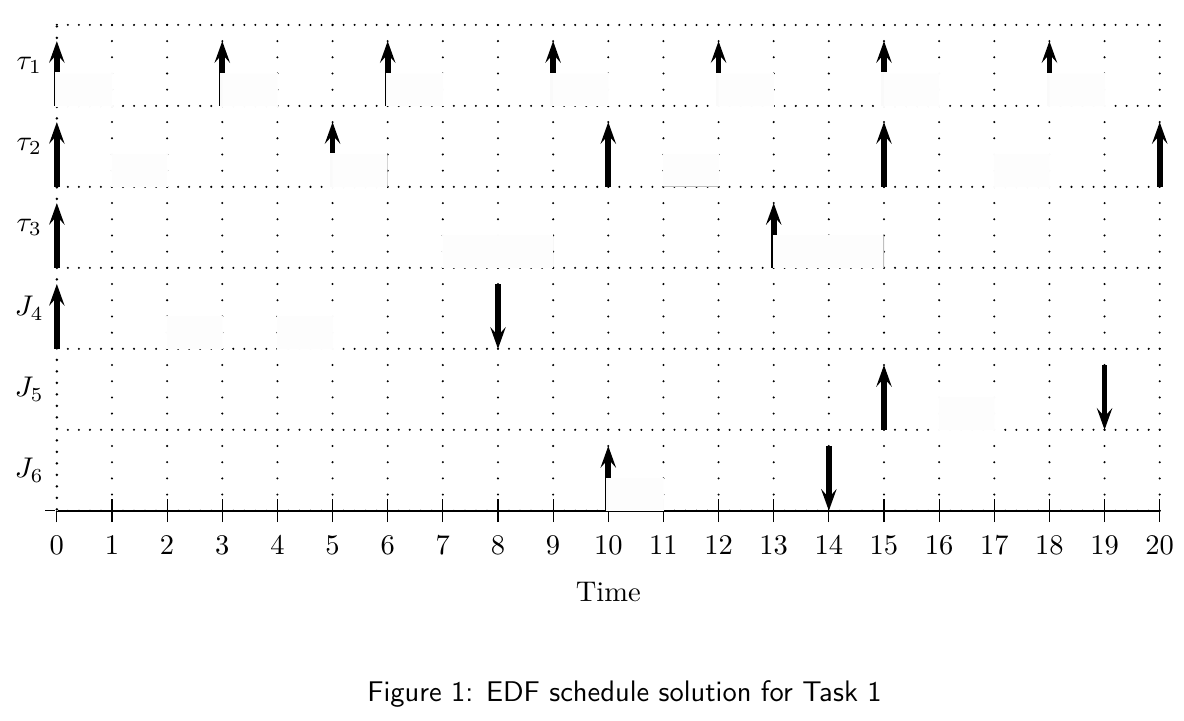
\includegraphics[height=0.6\paperheight]{./figures/1_sol_empty.png}
    \end{figure}
    \begin{figure}
      \centering
      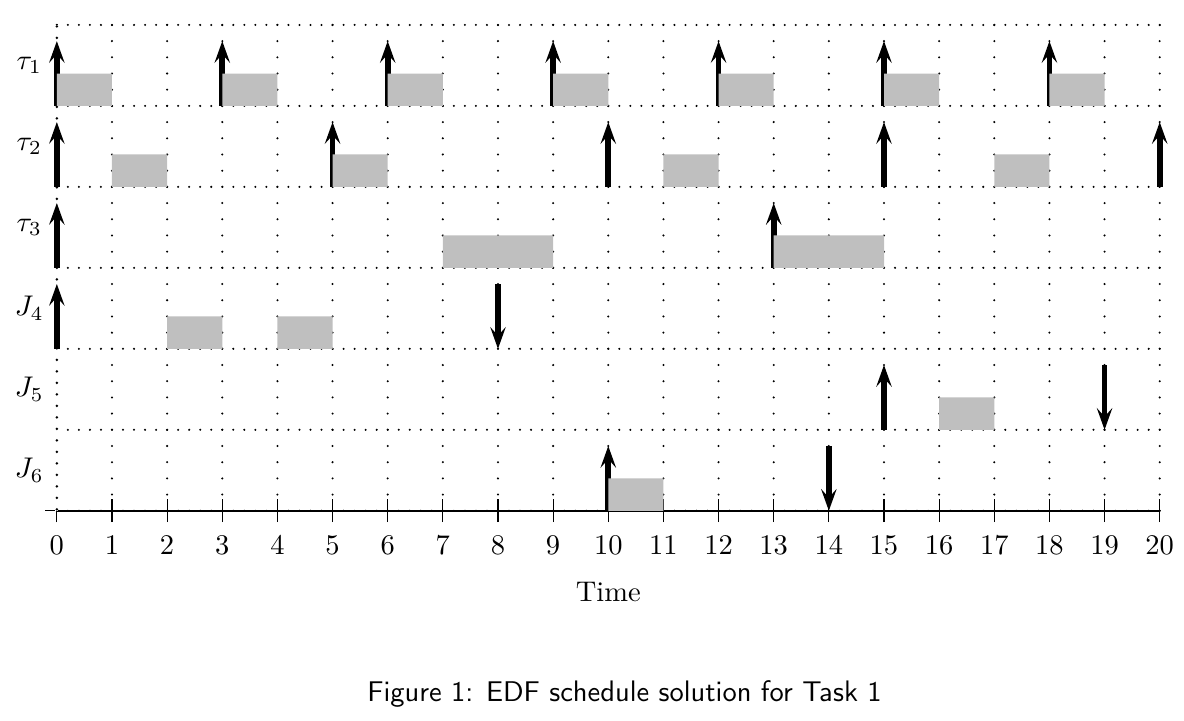
\includegraphics[height=0.6\paperheight]{./figures/1_sol.png}
    \end{figure}
\end{frame}
